%!TEX TS-program = xelatex
\documentclass[12pt,a4paper]{extarticle} 

\input{misc/_preamble.tex}
\addbibresource{misc/_references.bib}


\def\course{Теория игр}
\def\groupnumber{$\gamma$} %альфа -- первая группа (базовая), бета -- вторая группа, гамма -- третья группа
\date{7 августа 2026 года}  % Дедлайн
\def\lecturer{Сергей Кыльчик} % ФИО лектора (как на бейдже) 
\def\assist{Климент Шамаев} % ФИО ответственного составителя (как на бейдже)
%\def\listoknumber{1}  % Номер листка (если применимо, то раскомментировать)
\def\listokname{Модель Хотеллинга}
%\def\bonus{\textbf{Бонус за сданную задачу:} 5 HS€.} % Раскомментируйте, если за сдачу предусмотрен бонус.
\boolfalse{onlyorder} % Раскомментируйте, если задачи можно сдавать в любом порядке
 % Конец преамбулы, начало текста.
\begin{document}
\input{misc/_lesh2026.tex}
\z[Классика]{
Город $N$ представляет собой отрезок длины $1$, на котором равномерно распределены $120$ жителей. На краях города расположены фирмы. Функция издержек первой фирмы имеет вид $TC_1=20q_1$, функция издержек второй фирмы --- $TC_2=cq_2$. Каждый из жителей города покупает ровно единицу товара. Транспортные издержки равны расстоянию. Фирмы конкурируют, одновременно и независимо выбирая цены.
}{
\n Найдите все рыночные равновесия в зависимости для $c=20$.
\n Найдите все рыночные равновесия в зависимости от $c$.
}

\z[Товар $X$ в городе $M$]{
Улицы города $M$ имеют минималистичную структуру, изображённую на рисунке:
$$\includegraphics[scale=0.35]{Подборки/Микроэкономика/Fig 4 (1).png}$$
Числами подписаны \textit{длины} соответствующих улиц. Жители города равномерно расселены по улицам. Каждый из жителей хочет приобрести ровно единицу товара $X$. Товар $X$ могут продавать $n$ фирм. Цена на товар давно зафиксирована в строгом городском законодательстве и устраивает каждую из фирм. Поэтому, любая фирма максимизирует количество проданного товара $X$. Фирмы одновременно и независимо выбирают местоположения своих торговых точек в городе, после чего жители покупают товар $X$. Фирмы могут размещать сколько угодно торговых точек в одном месте. Каждый из жителей покупает товар в ближайшей к нему торговой точке. Если нескольким жителям безразлично между несколькими торговыми точками, считайте, что они делятся между ними поровну. Каждая из фирм открывает ровно одну торговую точку.\\
\textit{\small Равновесием называется ситуация, в которой ни одной из фирм не выгодно изменить местоположение своей торговой точки при фиксированных местоположениях точек других фирм.}
}{
\n Допустим, $n=2$. Верно ли, что ситуация, в которой несколько торговых точек стоят в одном месте, не является равновесием?
\n Допустим, $n=2$. Верно ли, что ситуация, в которой несколько торговых точек фирм стоят на одной улице, не является равновесием?
\n Допустим, $n=2$. Найдите все равновесия или докажите, что их не существует.
\n Допустим, $n=3$. Верно ли, что ситуация, в которой несколько торговых точек стоят в одном месте, не является равновесием?
\n Допустим, $n=3$. Верно ли, что ситуация, в которой несколько торговых точек стоят на одной улице, не является равновесием?
}

\z[Города и дороги]{
Страна $X$ состоит из трёх городов: М, С и К. За последние годы страна существенно урбанизировалась, поэтому население страны расположено исключительно в городах. Схема дорог страны изображена на карте:
\begin{center}
  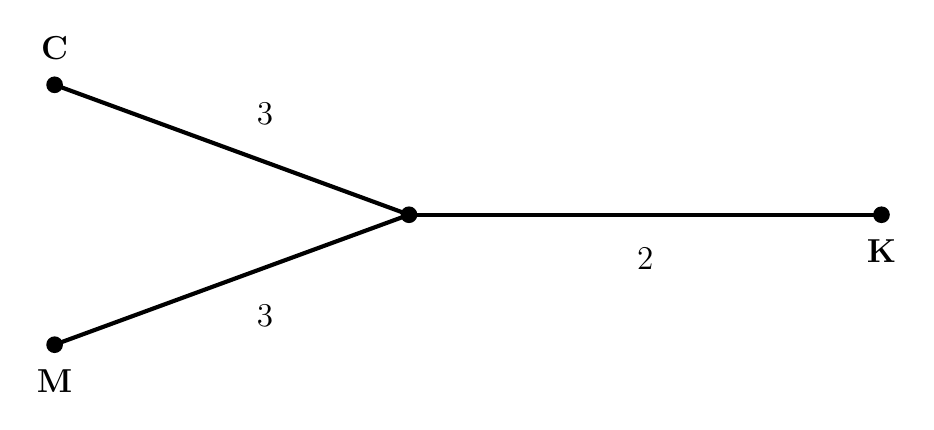
\begin{tikzpicture}[
    scale=1.5,
    line width=1.5pt,
    vertex label/.style={font=\bfseries\large}
  ]

    % 1. Координаты
    \coordinate (M) at (0,0);
    \coordinate (C) at (0,2.2);
    \coordinate (O) at (3,1.1);
    \coordinate (K) at (7,1.1);

    % 2. Линии и цифры
    \draw (C) -- node[above right=5pt] {\large 3} (O);
    \draw (M) -- node[below right=5pt] {\large 3} (O);
    \draw (O) -- node[below=8pt] {\large 2} (K);

    % 3. ТОЧКИ (Circle fill)
    \foreach \point in {M,C,O,K} {
        \filldraw[black] (\point) circle (1.5pt);
    }

    % 4. Буквы
    \node[vertex label, above=5pt] at (C) {C};
    \node[vertex label, below=5pt] at (M) {M};
    \node[vertex label, below=5pt] at (K) {K};

  \end{tikzpicture}
\end{center}

% $$\includegraphics[scale=0.7]{Олимпиада/img1.png}$$
Числами подписаны длины соответствующих дорог. Население города М составляет 4 жителя, население города С --- 3, население города К --- 2. Население страны может перемещаться только по дорогам.
В $3018$ году в стране станет возможно проведение крупного футбольного чемпионата, поэтому жители страны задумались о постройке футбольного стадиона. Так как в стране процветает демократия, жители решили принять решение о строительстве стадиона путём голосования. Система голосования устроена следующим образом:
\begin{enumerate}
    \item Правительства городов М и С называют точки $X_M$ и $X_C$ где-то на дорогах страны (возможно, в каком-то из городов). Будем называть эти точки кандидатами от соответствующих городов. Правительство каждого из городов стремится минимизировать расстояние вдоль дорог от собственного города до стадиона. Разные города могут выбрать одного кандидата, в таком случае он автоматически побеждает и следующие два этапа голосования пропускаются. Правительства действуют одновременно и независимо.
    \item Каждый из жителей отдает голос за одного из кандидатов. Жители голосуют за ближайшего к ним кандидата. Если множеству жителей безразлично между множеством кандидатов, голоса этих жителей делятся между соответствующими кандидатами поровну.
    \item Побеждает кандидат, набравший наибольшее число голосов. Информация о том, что происходит, если разные кандидаты набирают одинаковое число голосов, вам не понадобится.
    \item В точке-победителе строится стадион.
\end{enumerate}
Равновесным назовём такой набор кандидатов, что ни одно из правительств не имеет стимулов назначить другого кандидата от своего города.
}{
\n Отметьте на карте все возможные равновесные $X_M$ и $X_C$. Обоснуйте, почему данные $X_M$ и $X_C$ являются равновесными и почему других равновесий не существует.

Между городами С и М была построена дорога длины 2.

\n Докажите, что любая ситуация, в которой $X_M$ и $X_C$ лежат на дороге СМ (дорога СМ включает точки С и М) не является равновесием.
\n Докажите, что любая ситуация, в которой только $X_M$ лежит на дороге СМ (дорога СМ включает точки С и М) не является равновесием.
\n Осознав все трудности, связанные с работой системы голосования в таких условиях, жители решили изменить систему голосования.

Теперь стадион строится в точке на дорогах (возможно, в каком-то из городов), которая является \textit{победителем по Кондорсе}, то есть набирает больше половины голосов жителей будучи выставленной против любой другой точки на дорогах (возможно, в каком-то из городов). Жители по прежнему всегда голосуют за ближайшую точку и при безразличии делятся поровну.

Если победителя по Кондорсе не находится, стадион строится в городе М, если победителей по Кондорсе находится несколько, среди них выбирается точка, ближайшая к городу М. Найдите, в какой точке будет построен стадион.
}

\z[Это проще, чем вы думаете]{
Потребители некоторого товара живут на отрезке $[0,1]$. Потребители распределены по отрезку равномерно, то есть для всех $0\le a\le b\le 1$ доля жителей, живущих на отрезке $[a,b]$, равна $b-a$. Фирмы-производители товара расположены на краях города. Фирмы одновременно и независимо выбирают цены на свой товар. Издержки каждой из фирм имеет вид $TC=3q$. Каждый   потребитель покупает ровно единицу товара, минимизируя суммарные издержки на приобретение товара. Транспортные издержки потребителей равны пройденному расстоянию.
}{
\n Найдите спрос на продукцию каждой из фирм для \textit{любых} $P_1,P_2\ge 0$. 
\n Найдите рыночное равновесие. 
\n Государство вводит потолок цен на первую фирму на уровне $\overline{P_1}$ и потолок цен на вторую фирму на уровне $\overline{P_2}$. Найдите новое рыночное равновесие.
\n Найдите все общественно-оптимальные значения $\overline{P_1},\overline{P_2}$.
}

\z[Это сложнее, чем вы думаете]{
Город состоит из одной улицы длиной 1 км, на которой равномерно расположено все его население. В концах города расположены две фирмы: А и Б, которые производят хот-доги. Так как каждому человеку необходим хот-дог, вопрос стоит только в цене. Издержки человека на покупку хот-дога складываются из его цены и из того, сколько ему придется пройти до магазина. Если расстояние до магазина, где он купит хот-дог, составляет \( t \) километров, то он понесет дополнительные издержки, равные \( t \), в довесок к цене. Фирмы одновременно назначают свои цены. Издержки фирм равны \( 0 \). Найдите равновесные \( P_a \) и \( P_b \) в следующих ситуациях:

}{
\item Никаких дополнительных условий не накладывается

\item Та половина улицы, которая ближе к фирме Б, оказалась затоплена: издержки перемещения по ней оказываются в 2 раза выше.

}
\end{document}